\documentclass[a4paper]{report}
\usepackage{graphicx}
\usepackage{xspace,ifthen,epsfig}
\usepackage{cite}
\usepackage{color}
\usepackage{fancybox}
\usepackage{float}
\usepackage{subfigure}
\usepackage{longtable} 
\usepackage{tabularx} 
\usepackage{ltxtable} 
\usepackage{times}
\usepackage[table]{xcolor}
\usepackage{url}
\usepackage{listings}
\usepackage{amsmath}
\usepackage{dsfont}
\usepackage[american]{babel}
\usepackage[utf8]{inputenc}
\usepackage{fancyhdr}
\usepackage{booktabs}
\usepackage{tikz,pgfplots}
\usepackage{todonotes}
\usepackage{footmisc}
\usepackage{marvosym}
\usepackage{hyperref}

\usetikzlibrary{pgfplots.statistics}
\pgfplotsset{
  width=60mm,height=55mm,
  major grid style={thin,dotted,color=black!50},
  minor grid style={thin,dotted,color=black!50},
  grid,
  every axis/.append style={
    line width=0.5pt,
    tick style={
      line cap=round,
      thin,
      major tick length=4pt,
      minor tick length=2pt,
    },
  },
  /pgf/number format/1000 sep={},
  legend cell align=left,
  legend pos=north west,
  log y ticks with fixed point/.style={
      yticklabel={
        \pgfkeys{/pgf/fpu=true}
        \pgfmathparse{exp(\tick)}%
        \pgfmathprintnumber[fixed relative, precision=3]{\pgfmathresult}
        \pgfkeys{/pgf/fpu=false}
      }
  },
}

\begin{document}

\begin{figure}[H]
    % IMPORT-DATA urls data/uk-2007-05.urls.txt
    \centering
    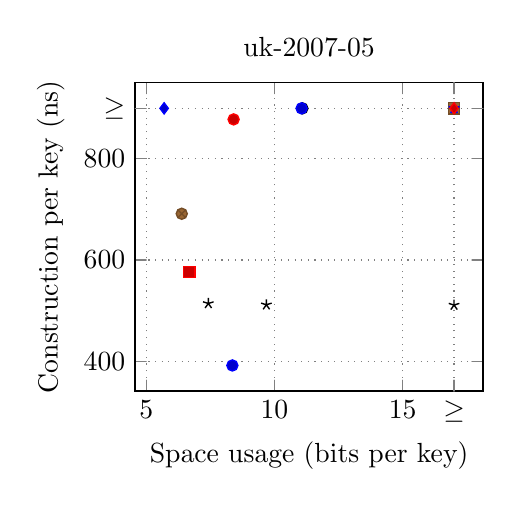
\begin{tikzpicture}
        \begin{axis}[
            title={uk-2007-05},
            xlabel={Space usage (bits per key)},
            ylabel={Construction per key (ns)},
            legend columns=3,
            only marks,
            extra x ticks={17},
            extra x tick labels={$\geq$},
            extra y ticks={900},
            extra y tick labels={$\geq$},
            legend to name=legendUrls,
          ]
          %% MULTIPLOT(name|title)
          %%   SELECT
          %%     MIN(bitsPerElement, 17) as x,
          %%     MIN(1000000.0*constructionTimeMilliseconds/N, 900) as y,
          %%     name,
          %%     name AS title
          %%   FROM urls
          %%   ORDER BY name,x
          \addplot coordinates { (8.35901,391.382) };
          \addlegendentry{CentroidHollowTrie};
          \addplot coordinates { (6.67972,575.741) };
          \addlegendentry{DirectRankStoring20230130};
          \addplot coordinates { (6.38508,691.477) };
          \addlegendentry{DirectRankStoring20230210};
          \addplot coordinates { (7.42151,513.907) (9.68466,511.329) (17,510.781) };
          \addlegendentry{HollowTrie};
          \addplot coordinates { (5.69871,900) };
          \addlegendentry{HollowTrieDistJava};
          \addplot coordinates { (8.40711,878.131) };
          \addlegendentry{HollowTrieJava};
          \addplot coordinates { (17,900) };
          \addlegendentry{LcpJava};
          \addplot coordinates { (11.0866,900) };
          \addlegendentry{PaCoTrieJava};
          \addplot coordinates { (17,900) (17,900) };
          \addlegendentry{PathDecomposedTrie};
          \addplot coordinates { (17,900) };
          \addlegendentry{VLLcpJava};
          \addplot coordinates { (11.0581,900) };
          \addlegendentry{VLPaCoTrieJava};
        \end{axis}
    \end{tikzpicture}
    \hfill
    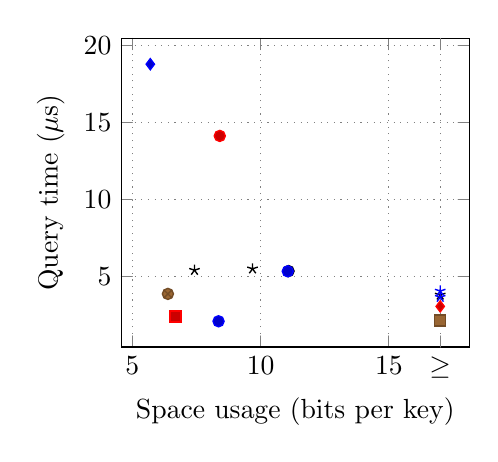
\begin{tikzpicture}
        \begin{axis}[
            title={},
            xlabel={Space usage (bits per key)},
            ylabel={Query time ($\mu$s)},
            only marks,
            extra x ticks={17},
            extra x tick labels={$\geq$},
          ]
          %% MULTIPLOT(name|title)
          %%   SELECT
          %%     MIN(bitsPerElement, 17) as x,
          %%     1000.0*queryTimeMilliseconds/numQueries as y,
          %%     name,
          %%     name AS title
          %%   FROM urls
          %%   ORDER BY name,x
          \addplot coordinates { (8.35901,2.1225) };
          \addlegendentry{CentroidHollowTrie};
          \addplot coordinates { (6.67972,2.429) };
          \addlegendentry{DirectRankStoring20230130};
          \addplot coordinates { (6.38508,3.9) };
          \addlegendentry{DirectRankStoring20230210};
          \addplot coordinates { (7.42151,5.439) (9.68466,5.5295) (17,3.83) };
          \addlegendentry{HollowTrie};
          \addplot coordinates { (5.69871,18.8085) };
          \addlegendentry{HollowTrieDistJava};
          \addplot coordinates { (8.40711,14.152) };
          \addlegendentry{HollowTrieJava};
          \addplot coordinates { (17,2.1705) };
          \addlegendentry{LcpJava};
          \addplot coordinates { (11.0866,5.3805) };
          \addlegendentry{PaCoTrieJava};
          \addplot coordinates { (17,3.6875) (17,4.0865) };
          \addlegendentry{PathDecomposedTrie};
          \addplot coordinates { (17,3.0865) };
          \addlegendentry{VLLcpJava};
          \addplot coordinates { (11.0581,5.3655) };
          \addlegendentry{VLPaCoTrieJava};

          \legend{};
        \end{axis}
    \end{tikzpicture}

    % IMPORT-DATA titles data/trec-title.terms.txt
    \centering
    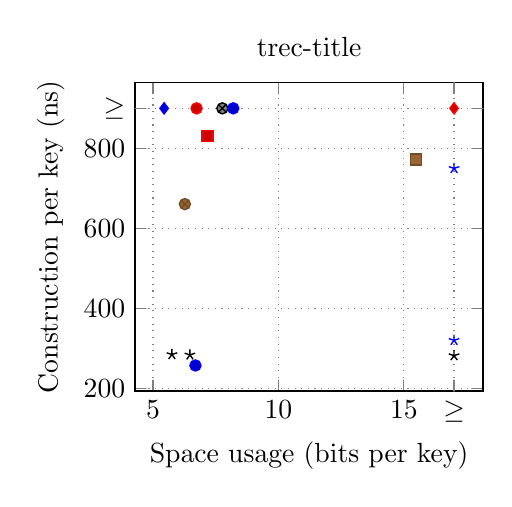
\begin{tikzpicture}
        \begin{axis}[
            title={trec-title},
            xlabel={Space usage (bits per key)},
            ylabel={Construction per key (ns)},
            legend style={at={(1.03,0.5)},anchor=west},
            legend columns=4,
            only marks,
            extra x ticks={17},
            extra x tick labels={$\geq$},
            extra y ticks={900},
            extra y tick labels={$\geq$},
          ]
          %% MULTIPLOT(name|title)
          %%   SELECT
          %%     MIN(bitsPerElement, 17) as x,
          %%     MIN(1000000.0*constructionTimeMilliseconds/N, 900) as y,
          %%     name,
          %%     name AS title
          %%   FROM titles
          %%   ORDER BY name,x
          \addplot coordinates { (6.69053,257.307) };
          \addlegendentry{CentroidHollowTrie};
          \addplot coordinates { (7.16934,831.228) };
          \addlegendentry{DirectRankStoring20230130};
          \addplot coordinates { (6.26808,660.603) };
          \addlegendentry{DirectRankStoring20231002};
          \addplot coordinates { (5.75304,284.68) (6.4705,283.767) (17,281.942) };
          \addlegendentry{HollowTrie};
          \addplot coordinates { (5.44223,900) };
          \addlegendentry{HollowTrieDistJava};
          \addplot coordinates { (6.73464,900) };
          \addlegendentry{HollowTrieJava};
          \addplot coordinates { (15.4768,771.92) };
          \addlegendentry{LcpJava};
          \addplot coordinates { (7.76357,900) };
          \addlegendentry{PaCoTrieJava};
          \addplot coordinates { (17,320.265) (17,750.021) };
          \addlegendentry{PathDecomposedTrie};
          \addplot coordinates { (17,900) };
          \addlegendentry{VLLcpJava};
          \addplot coordinates { (8.19657,900) };
          \addlegendentry{VLPaCoTrieJava};

          \legend{};
        \end{axis}
    \end{tikzpicture}
    \hfill
    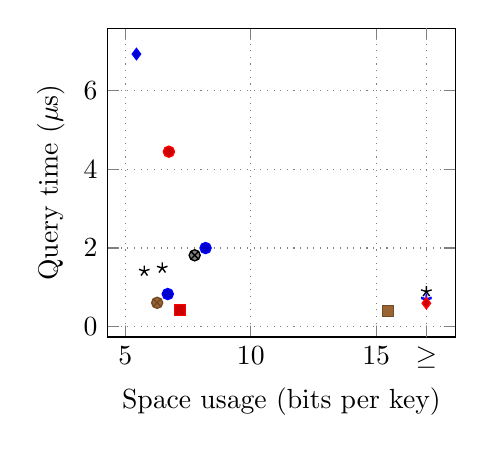
\begin{tikzpicture}
        \begin{axis}[
            title={},
            xlabel={Space usage (bits per key)},
            ylabel={Query time ($\mu$s)},
            only marks,
            extra x ticks={17},
            extra x tick labels={$\geq$},
          ]
          %% MULTIPLOT(name|title)
          %%   SELECT
          %%     MIN(bitsPerElement, 17) as x,
          %%     1000.0*queryTimeMilliseconds/numQueries as y,
          %%     name,
          %%     name AS title
          %%   FROM titles
          %%   ORDER BY name,x
          \addplot coordinates { (6.69053,0.832) };
          \addlegendentry{CentroidHollowTrie};
          \addplot coordinates { (7.16934,0.428) };
          \addlegendentry{DirectRankStoring20230130};
          \addplot coordinates { (6.26808,0.61) };
          \addlegendentry{DirectRankStoring20231002};
          \addplot coordinates { (5.75304,1.414) (6.4705,1.492) (17,0.894) };
          \addlegendentry{HollowTrie};
          \addplot coordinates { (5.44223,6.916) };
          \addlegendentry{HollowTrieDistJava};
          \addplot coordinates { (6.73464,4.441) };
          \addlegendentry{HollowTrieJava};
          \addplot coordinates { (15.4768,0.397) };
          \addlegendentry{LcpJava};
          \addplot coordinates { (7.76357,1.814) };
          \addlegendentry{PaCoTrieJava};
          \addplot coordinates { (17,0.676) (17,0.7075) };
          \addlegendentry{PathDecomposedTrie};
          \addplot coordinates { (17,0.598) };
          \addlegendentry{VLLcpJava};
          \addplot coordinates { (8.19657,1.998) };
          \addlegendentry{VLPaCoTrieJava};

          \legend{};
        \end{axis}
    \end{tikzpicture}

    % IMPORT-DATA text data/trec-text.terms.txt
    \centering
    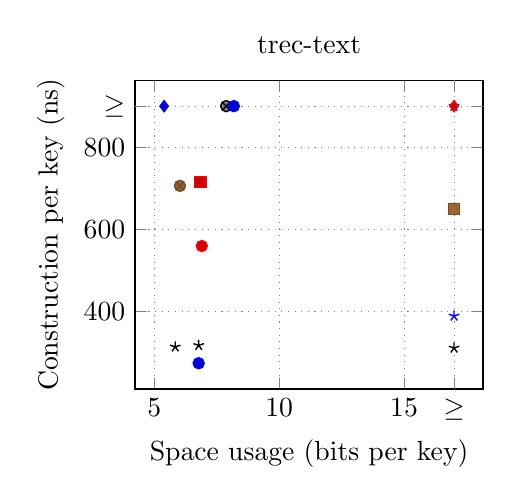
\begin{tikzpicture}
        \begin{axis}[
            title={trec-text},
            xlabel={Space usage (bits per key)},
            ylabel={Construction per key (ns)},
            legend style={at={(1.03,0.5)},anchor=west},
            legend columns=4,
            only marks,
            extra x ticks={17},
            extra x tick labels={$\geq$},
            extra y ticks={900},
            extra y tick labels={$\geq$},
          ]
          %% MULTIPLOT(name|title)
          %%   SELECT
          %%     MIN(bitsPerElement, 17) as x,
          %%     MIN(1000000.0*constructionTimeMilliseconds/N, 900) as y,
          %%     name,
          %%     name AS title
          %%   FROM text
          %%   ORDER BY name,x
          \addplot coordinates { (6.77934,273.355) };
          \addlegendentry{CentroidHollowTrie};
          \addplot coordinates { (6.84487,715.352) };
          \addlegendentry{DirectRankStoring20230130};
          \addplot coordinates { (6.02976,705.715) };
          \addlegendentry{DirectRankStoring20230210};
          \addplot coordinates { (5.84184,313.307) (6.77952,316.949) (17,310.582) };
          \addlegendentry{HollowTrie};
          \addplot coordinates { (5.39703,900) };
          \addlegendentry{HollowTrieDistJava};
          \addplot coordinates { (6.90449,559.071) };
          \addlegendentry{HollowTrieJava};
          \addplot coordinates { (17,649.214) };
          \addlegendentry{LcpJava};
          \addplot coordinates { (7.87968,900) };
          \addlegendentry{PaCoTrieJava};
          \addplot coordinates { (17,388.651) (17,900) };
          \addlegendentry{PathDecomposedTrie};
          \addplot coordinates { (17,900) };
          \addlegendentry{VLLcpJava};
          \addplot coordinates { (8.18601,900) };
          \addlegendentry{VLPaCoTrieJava};

          \legend{};
        \end{axis}
    \end{tikzpicture}
    \hfill
    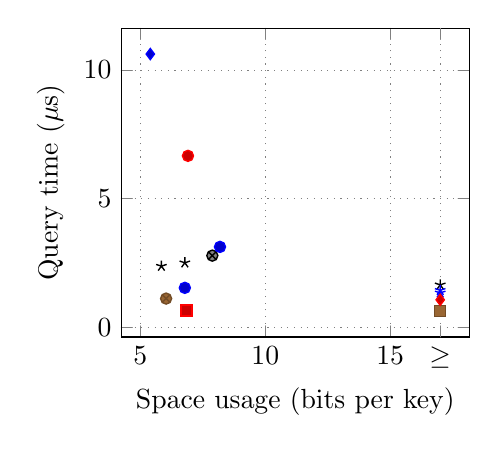
\begin{tikzpicture}
        \begin{axis}[
            title={},
            xlabel={Space usage (bits per key)},
            ylabel={Query time ($\mu$s)},
            only marks,
            extra x ticks={17},
            extra x tick labels={$\geq$},
          ]
          %% MULTIPLOT(name|title)
          %%   SELECT
          %%     MIN(bitsPerElement, 17) as x,
          %%     1000.0*queryTimeMilliseconds/numQueries as y,
          %%     name,
          %%     name AS title
          %%   FROM text
          %%   ORDER BY name,x
          \addplot coordinates { (6.77934,1.537) };
          \addlegendentry{CentroidHollowTrie};
          \addplot coordinates { (6.84487,0.6515) };
          \addlegendentry{DirectRankStoring20230130};
          \addplot coordinates { (6.02976,1.12) };
          \addlegendentry{DirectRankStoring20230210};
          \addplot coordinates { (5.84184,2.3805) (6.77952,2.511) (17,1.654) };
          \addlegendentry{HollowTrie};
          \addplot coordinates { (5.39703,10.621) };
          \addlegendentry{HollowTrieDistJava};
          \addplot coordinates { (6.90449,6.666) };
          \addlegendentry{HollowTrieJava};
          \addplot coordinates { (17,0.6295) };
          \addlegendentry{LcpJava};
          \addplot coordinates { (7.87968,2.789) };
          \addlegendentry{PaCoTrieJava};
          \addplot coordinates { (17,1.341) (17,1.4405) };
          \addlegendentry{PathDecomposedTrie};
          \addplot coordinates { (17,1.071) };
          \addlegendentry{VLLcpJava};
          \addplot coordinates { (8.18601,3.128) };
          \addlegendentry{VLPaCoTrieJava};

          \legend{};
        \end{axis}
    \end{tikzpicture}

    \begin{tikzpicture}
        \ref*{legendUrls}
    \end{tikzpicture}
\end{figure}

\end{document}
